         \chapter{Chemiese binding}\fancyfoot[LO,RE]{Chemie: Stof en Materie}
    \setcounter{figure}{1}
    \setcounter{subfigure}{1}
    \label{m38704*cid1}
            \section{Inleiding}
            \nopagebreak

As jy na alles rondom jou kyk en waarvan dit gemaak is, sal jy besef dat atome selde op hul  eie bestaan. Meer dikwels bestaan die dinge rondom ons ​​uit verskillende atome wat saamgevoeg is. Dit staan bekend as \textbf{chemiese binding}. Chemiese binding is een van die belangrikste prosesse in chemie, want dit maak die vorming van allerhande verskillende molekules en kombinasies van atome moontlik, wat dan deel uitmaak van die voorwerpe in die komplekse w\^{e}reld rondom ons. \par 
\chapterstartvideo{VPawb}
    \label{m38704*cid4}
            \subsection*{Wat gebeur wanneer atome bind?}
            \nopagebreak
      \label{m38704*id138842} 'n \textbf{Chemiese binding} word gevorm wanneer atome bymekaar gehou word deur aantrekkingskragte. Hier\-die aantrekkingskragte ontstaan wanneer elektrone tussen atome gedeel word, of wanneer elektrone tussen atome wat betrokke is by die binding, uitgeruil word. Die deel of die uitruil van elektrone vind plaas sodat die buitenste energievlakke van die atome wat betrokke is, gevul kan word en die atome dan meer stabiel sal wees. Wanneer 'n elektron \textbf{gedeel} word, sal dit tyd spandeer binne die elektronorbitale van beide atome. As 'n elektron \textbf{uitgeruil} word, beteken dit dat dit oorgedra word van een atoom na 'n ander, met ander woorde, een atoom kry 'n elektron by, terwyl  'n ander atoom  'n elektron verloor.\par 
\label{m38704*fhsst!!!underscore!!!id83}
\Definition{Chemiese binding} { 'n Chemiese binding is die fisiese proses wat veroorsaak dat atome en molekules mekaar aantrek en saamgevoeg word tot meer stabiele chemiese verbindings.} 
      \label{m38704*id138909}Die tipe binding wat gevorm word, hang af van die elemente wat betrokke is. In hierdie hoofstuk
sal ons kyk na drie tipes van chemiese binding: \textbf{kovalente}-, \textbf{ioniese}- en \textbf{metaal}binding.\par 
      \label{m38704*id138929}
Jy moet onthou dat dit die \textsl{valenselektrone} is wat by binding betrokke is en dat atome altyd sal probeer om hul buitenste energievlakke te vul, sodat hulle meer stabiel kan wees (of meer kan wees soos die edelgasse, wat baie stabiel is en nie met ander atome reageer nie).\par 
 
\section{Lewisstrukture}
    \nopagebreak

\textbf{Lewisnotasie} gebruik kolletjies en kruisies om die \textbf{valenselektrone} by verskillende atome voor te stel. Die chemiese simbool van die element word gebruik om die kern en die \textsl{binneste elektrone} van die atoom te verteenwoordig. Om die valenselektrone te identifiseer, kyk ons na die laaste/hoogste energievlak in die atoom se elektronstruktuur (hoofstuk~\ref{chap:atom}). Die elektronstruktuur van byvoorbeeld silikon kan geskryf word as: $1\text{s}^{2}2\text{s}^{2}2\text{p}^{6}3\text{s}^{2}3\text{p}^{2}$ of $\text{[Ne]}3\text{s}^{2}3\text{p}^{2}$. Die laaste energievlak is die 3de een is, en dit bevat 4 elektrone. Dit is die valenselektrone.
\Tip{As ons  die verkorte  elektronkonfigurasie  neerskryf, kan ons maklik valenselektrone raaksien.}
 \par 
So, byvoorbeeld, kan 'n waterstofatoom voorgestel word as volg:  
% \begin{center}
\scalebox{0.8}{
\begin{pspicture}(1.5,1.5)(2.5,2.1)
%\psgrid[gridcolor=lightgray]
\rput(2,2){\Large \textbf{$\text{H}$}}
\rput(2.5,2){$\bullet$}
\end{pspicture}
}
% \end{center}

 'n Chlooratoom sal lyk as volg: 
% \begin{center}
\scalebox{0.8}{
\begin{pspicture}(-1,-0.6)(2,0.4)
%\psgrid[gridcolor=lightgray]
\rput(1,0){\Large \textbf{$\text{Cl}$}}
\uput{9pt}[d](1,0){$\times$ $\times$}
\rput{90}(1,0){\uput{9pt}[d](0,0){$\times$ $\times$}}
\rput{180}(1,0){\uput{9pt}[d](0,0){$\times$ $\times$}}
\rput{270}(1,0){\uput{9pt}[d](0,0){$\times$}}
\end{pspicture}
}
% \end{center}

 'n Molekule van waterstofchloried kan as volg voorgestel word:
\begin{center}
\scalebox{0.8}{
\begin{pspicture}(-1,-0.6)(2,0.6)
%\psgrid[gridcolor=lightgray]
\rput(1,0){\Large \textbf{$\text{Cl}$}}
\uput{9pt}[d](1,0){$\times$ $\times$}
\rput{90}(1,0){\uput{9pt}[d](0,0){$\times$ $\times$}}
\rput{180}(1,0){\uput{9pt}[d](0,0){$\times$ $\times$}}
\rput{270}(1,0){\uput{9pt}[d](0,0){$\times$ $\bullet$}}
\rput(0,0){\Large \textbf{$\text{H}$}}
\end{pspicture}
}
\end{center}

      \par 
      \label{m38701*id140178}Die kolletjie en kruisie tussen die twee atome verteenwoordig die elektronpaar wat gedeel word in hierdie kovalente binding.\par 
Tabel~\ref{tab:lewis} gee 'n paar verdere voorbeelde van Lewisdiagramme.
\begin{table}[H]
 \begin{center}
  \begin{tabular}{|l|l|l|} \hline
   Jodium & $\text{I}_2$ & 
\begin{pspicture}(-2,-0.4)(4,0.4)
%\psgrid[gridcolor=gray]
\rput(1,0){\Large \textbf{$\text{I}$}}
\uput{9pt}[d](1,0){$\times$ $\times$}
\rput{180}(1,0){\uput{9pt}[d](0,0){$\times$ $\times$}}
\rput{270}(1,0){\uput{9pt}[d](0,0){$\times$ $\times$}}
\rput(2,0){\Large \textbf{$\text{I}$}}
\uput{9pt}[d](2,0){$\bullet$ $\bullet$}
\rput{90}(2,0){\uput{9pt}[d](0,0){$\bullet$ $\bullet$}}
\rput{180}(2,0){\uput{9pt}[d](0,0){$\bullet$ $\bullet$}}
\rput{270}(2,0){\uput{9pt}[d](0,0){$\times$ $\bullet$}}
\end{pspicture} \\ \hline
   Water & $\text{H}_{2}\text{O}$ & 
\begin{pspicture}(-0.2,-0.4)(2,0.4)
%\psgrid[gridcolor=gray]
\rput(0.1,0){\Large \textbf{$\text{H}$}}
\rput(1,0){\Large \textbf{$\text{O}$}}
\uput{9pt}[d](1,0){$\times$ $\bullet$}
\rput{90}(1,0){\uput{9pt}[d](0,0){$\times$ $\times$}}
\rput{180}(1,0){\uput{9pt}[d](0,0){$\times$ $\times$}}
\rput{270}(1,0){\uput{9pt}[d](0,0){$\times$ $\bullet$}}
\rput(1,-0.8){\Large \textbf{$\text{H}$}}
\end{pspicture} \\ \hline
   Koolstofdioksied & $\text{CO}_2$ &
\begin{pspicture}(-2,-0.4)(4,0.4)
%\psgrid[gridcolor=gray]
\rput(0.1,0){\Large \textbf{$\text{O}$}}
\rput{220}(.1,0){\uput{9pt}[d](0,0){$\bullet$ $\bullet$}}
\rput{320}(.1,0){\uput{9pt}[d](0,0){$\bullet$ $\bullet$}}
\rput{90}(0,0){\uput{9pt}[d](0,0){$\bullet$ $\bullet$ }}
\rput(1,0){\Large \textbf{$\text{C}$}}
\rput{270}(1,0){\uput{9pt}[d](0,0){$\times$ $\times$}}
\rput{90}(1,0){\uput{9pt}[d](0,0){$\times$ $\times$ }}
\rput(2,0){\Large \textbf{$\text{O}$}}
\rput{40}(2,0){\uput{9pt}[d](0,0){$\bullet$ $\bullet$}}
\rput{140}(2,0){\uput{9pt}[d](0,0){$\bullet$ $\bullet$}}
\rput{270}(2,0){\uput{9pt}[d](0,0){$\bullet$ $\bullet$ }}
\end{pspicture} \\ \hline
Waterstofsianied & $\text{HCN}$ &
\begin{pspicture}(-2,-0.4)(4,0.4)
%\psgrid[gridcolor=gray]
\rput(0.1,0){\Large \textbf{$\text{H}$}}
\rput(1,0){\Large \textbf{$\text{C}$}}
\rput{270}(1,0){\uput{9pt}[d](0,0){$\times$ $\bullet$}}
\rput{90}(1,0){\uput{9pt}[d](0,0){$\times$ $\times$ $\times$}}
\rput(2,0){\Large \textbf{$\text{N}$}}
\rput{90}(2,0){\uput{9pt}[d](0,0){$\bullet$ $\bullet$}}
\rput{270}(2,0){\uput{9pt}[d](0,0){$\bullet$ $\bullet$ $\bullet$}}
\end{pspicture} \\ \hline  
  \end{tabular}
\caption{Lewisdiagramme vir 'n paar eenvoudige molekules}
\label{tab:lewis}
 \end{center}
\end{table}
            

Jy sal sien hoe ons die dubbele band koolstofdioksied in Lewisnotasie voorgestel het. Aangesien daar twee bande tussen suurstofatome en die koolstofatoom is, word hulle deur twee pare valenselektrone aanmekaar gekoppel. Op soortgelyke wyse word 'm drievoudige band in waterstofsianied aangedui.

\begin{exercises}{Lewisstrukture}
{
            \nopagebreak
      \label{m38701*id140889}\begin{enumerate}[noitemsep, label=\textbf{\arabic*}. ] 
            \label{m38701*uid23}\item Gebruik Lewisdiagramme om 'n voorstelling van elk van die volgende \textbf{atome} te maak:
\label{m38701*id140910}\begin{enumerate}[noitemsep, label=\textbf{\alph*}. ] 
            \label{m38701*uid24}\item berillium
\label{m38701*uid25}\item kalsium
\label{m38701*uid26}\item litium
\end{enumerate}
                \label{m38701*uid27}\item  Stel elk van die volgende \textbf{molekules} voor met behulp van Lewisdiagramme:
\label{m38701*id140969}\begin{enumerate}[noitemsep, label=\textbf{\alph*}. ] 
            \label{m38701*uid28}\item broom gas ($\text{Br}{}_{2}$)
\label{m38701*uid29}\item koolstofdioksied ($\text{CO}{}_{2}$)
\end{enumerate}
Watter van hierdie twee molekules bevat 'n dubbelbinding?
\label{m38701*uid31}\item Twee chemiese reaksies word hieronder beskryf.
\label{m38701*id141048}\begin{itemize}[noitemsep]
            \label{m38701*uid32}\item stikstof en waterstof reageer om $\text{NH}_{3}$ vorm
\label{m38701*uid33}\item koolstof en waterstof bind om 'n molekule $\text{CH}_{4}$ te vorm
\end{itemize}
Vir elkeen van die reaksies, verskaf die volgende inligting:
\label{m38701*id141106}\begin{enumerate}[noitemsep, label=\textbf{\alph*}. ] 
\item die aantal elektrone in die buitenste energievlak
\label{m38701*uid35}\item die Lewis-struktuur van die produk wat gevorm word
\label{m38701*uid37}\item die naam van die produk
\end{enumerate}
                \label{m38701*uid38}\item 'n Chemiese verbinding het die volgende Lewisnotasie:
    \setcounter{subfigure}{0}
	\begin{figure}[H] % horizontal\label{m38701*id141174}
\begin{center}
\scalebox{.8}{
\begin{pspicture}(1,-1)(2,0.4)
%\psgrid[gridcolor=gray]
\rput(0.1,0){\Large \textbf{X}}
\rput(1,0){\Large \textbf{Y}}
\uput{9pt}[d](1,0){$\times$ $\bullet$}
\rput{90}(1,0){\uput{9pt}[d](0,0){$\times$ $\times$}}
\rput{180}(1,0){\uput{9pt}[d](0,0){$\times$ $\times$}}
\rput{270}(1,0){\uput{9pt}[d](0,0){$\times$ $\bullet$}}
\rput(1,-0.8){\Large \textbf{H}}
\end{pspicture}
}
\end{center}
 \end{figure}       \label{m38701*id141181}\begin{enumerate}[noitemsep, label=\textbf{\alph*}. ] 
            \label{m38701*uid39}\item Hoeveel valenselektrone het element $\text{Y}$?
\label{m38701*uid40}\item Wat is die valensie van element $\text{Y}$?
\label{m38701*uid41}\item Wat is die valensie van element $\text{X}$?
\label{m38701*uid42}\item Hoeveel kovalente bindings is in die molekule?
\label{m38701*uid43}\item Stel 'n naam voor vir die elemente $\text{X}$ en $\text{Y}$.
\end{enumerate}
                \end{enumerate}

% Automatically inserted shortcodes - number to insert 4
\par \practiceinfo
\par \begin{tabular}[h]{cccccc}
% Question 1
(1.)	025q	&
% Question 2
(2.)	025r	&
% Question 3
(3.)	025s	&
% Question 4
(4.)	025t	&
\end{tabular}
% Automatically inserted shortcodes - number inserted 4
}
\end{exercises}


            \section{Kovalente binding}
            \nopagebreak
            \label{m38704*uid6}
            \subsection*{Die aard van kovalente bindings}
            \nopagebreak
        \label{m38704*id138956}
Kovalente bindings kom voor tussen die atome van \textbf{nie-metale}. Die buitenste orbitale van die atome oorvleuel so dat die ongepaarde elektrone by elk van die bindingsatome gedeel kan word. Die buitenste energievlakke van die atome wat bind, word gevul deurdat die orbitale oorvleuel. Die gedeelde elektrone beweeg in die orbitale rondom \textbf{beide} atome. Soos hulle beweeg, is daar 'n aantrekkingskrag tussen hierdie negatief gelaaide elektrone en die positief gelaaide kerne en hierdie krag hou die atome saam binne 'n kovalente binding.\par 

\mindsetvid{sharing elektrons}{VPaxf}

\label{m38704*fhsst!!!underscore!!!id94}
\Definition{Kovalente binding} {Kovalente binding is 'n vorm van chemiese binding waar elektronpare tussen atome gedeel word.} 
\label{m38704*id139505}Jy sal opmerk het in tabel~\ref{tab:lewis} dat die aantal elektrone wat by binding betrokke is, wissel tussen atome. Ons kan die volgende s\^{e}:
\begin{itemize}
 \item 'n \textbf{enkele kovalente} binding word gevorm wanneer twee elektrone gedeel word tussen dieselfde twee atome, een elektron vanaf elke atoom. 
 \item 'n \textbf{dubbele kovalente} binding gevorm word wanneer vier elektrone gedeel word tussen dieselfde twee atome, twee elektrone vanaf elke atoom.
 \item 'n \textbf{driedubbele kovalente} binding word gevorm wanneer ses elektrone gedeel word tussen dieselfde twee atome, drie elektrone vanaf elke atoom.
\end{itemize}
Jy sal ook opmerk dat verbindings 'n mengsel van enkel-, dubbel en driedubbele bindings kan bevat en dat 'n atoom verskeie bindings kan vorm. Met ander woorde, 'n atoom deel nie altyd sy valenselektrone slegs met een enkele ander atoom nie, maar kan valenselektrone deel met  'n hele paar verskillende atome.\\
Ons s\^{e} dat die \textbf{valensie} van atome verskillend is. 
\Definition{Valensie}{Die aantal elektrone in die buitenste vlak van 'n atoom wat gebruik kan word om bindings met ander atome te vorm.}

\Tip{Daar is 'n verwantskap tussen die valensie van 'n element en sy posisie op die periodieke tabel. Vir die elemente in groepe 1 en 2 is die valensie die groep nommer. Vir die elemente in groepe 13-18 is die valensie die groepnommer minus 10. Vir oorgangsmetale varieer die valensie. In hierdie gevalle word die valensie met 'n romeinse syfer na die e\-le\-ment aangedui, byvoorbeeld yster(III)chloried.}

\label{m38704*id138991}Hier is 'n paar voorbeelde. Onthou dat slegs die \textbf{valenselektrone} betrokke is by binding, so wanneer diagramme geteken word om te wys wat tydens binding gebeur, word slegs hierdie elektrone aangetoon. \par 
\label{m38704*secfhsst!!!underscore!!!id98} 


\begin{wex}{Kovalente binding}{Hoe bind waterstof- en chlooratome  kovalent om  'n molekule van waterstofchloried te vorm?}
{
\westep{Bepaal die elektronkonfigurasie van elk van die bindingsatome.}
'n Chlooratoom het 17 elektrone en 'n elektronkonfigurasie van $\text{[Ne]}3\text{s}^{2}3\text{p}^{5}$.  'n Waterstofatoom het net 1 elektron en 'n elektronkonfigurasie van $1\text{s}^{1}$.


\westep{Bepaal hoeveel van die elektrone is gepaar of ongepaar.}
Chloor het 7 valenselektrone. Een van hierdie elektrone is ongepaar. Waterstof het 1 valens elektron en dit is ongepaar.

\westep{Werk uit hoe die elektrone gedeel word}
Die waterstofatoom benodig een ekstra elektron om sy buitenste energievlak te voltooi. Die chlooratoom het ook een elektron nodig om sy buitenste energievlak te voltooi. Daar moet dus  'n elektronpaar gedeel word deur die twee atome.  'n Enkele kovalente binding sal gevorm word.
\begin{figure}[H]
\begin{center}
\scalebox{0.6}{
\begin{pspicture}(-7,-4.5)(7,1.5)
%\psgrid
\rput(-3.5,-1.8){\textbf{+}}
% Lower left
\uput[u](-5,-2){
\pscircle(0,0){1}
\qdisk(0.83,0.45){0.2}
\pscircle(3.5,0){1.5}
\uput{0}[u](0,-.2){\scalebox{2}{$\text{H}$}}

\rput(1.25,0){ 
\uput[d](0.83,-0.1){ \scalebox{2}{x}}
\uput{0.01}[l](2.25,1.5){ \scalebox{2}{x}}
\uput{0.01}[r](2.25,1.5){ \scalebox{2}{x}}
\uput[u](3.65,0){ \scalebox{2}{x}}
\uput[d](3.65,0){ \scalebox{2}{x}}
\uput{0.01}[l](2.25,-1.45){ \scalebox{2}{x}}
\uput{0.01}[r](2.25,-1.45){ \scalebox{2}{x}} 
\uput{0}[u](2.25,-.2){\scalebox{2}{$\text{Cl}$}}
}
}

% \psline{->}(0.5,2)(1.5,2)
\psline{->}(0.65,-2)(1.65,-2)

% Lower right
\uput[u](3,-2){
\pscircle(0,0){1}
\pscircle(2.25,0){1.5}
\qdisk(0.83,0.45){0.2}
\uput{0}[u](0,-.2){\scalebox{2}{$\text{H}$}}

\uput[d](0.83,-0.1){ \scalebox{2}{x}}
\uput{0.01}[l](2.25,1.5){ \scalebox{2}{x}}
\uput{0.01}[r](2.25,1.5){ \scalebox{2}{x}}
\uput[u](3.65,0){ \scalebox{2}{x}}
\uput[d](3.65,0){ \scalebox{2}{x}}
\uput{0.01}[l](2.25,-1.45){ \scalebox{2}{x}}
\uput{0.01}[r](2.25,-1.45){ \scalebox{2}{x}} 
\uput{0}[u](2.25,-.2){\scalebox{2}{$\text{Cl}$}}
}
\end{pspicture}
}
\end{center}
% \caption{Covalent bonding in a molecule of hydrogen chloride}
% \label{fig:bonding:hydrogen chloride}
 \end{figure}
}
\end{wex}
\begin{wex}{Kovalente binding met veelvoudige bindings }{
 %problem
Hoe bind stikstof- en waterstof- atome om 'n molekule van ammoniak ($\text{NH}{}_{3}$) te vorm? 
}
{
%solution
\westep{Bepaal die elektronkonfigurasie} 
 'n Stikstofatoom  het 7 elektrone en 'n elektronkonfigurasie van $\text{[He]}2\text{s}^{2}2\text{p}^{3}$. 'n Waterstofatoom het slegs een elektron en  'n elektronkonfigurasie van $1\text{s}^{1}$.
        \westep{Bepaal die aantal valenselektrone}  
Stikstof het 5 valenselektrone waarvan 3 ongepaar is. Waterstof het 1 valenselektron en dit is ongepaar.
        \westep{Stel vas hoe die elektrone gedeel word} 
Elke waterstofatoom benodig een ekstra elektron om sy valensenergievlak te voltooi. Die stikstofatoom benodig drie ekstra elektrone om sy valens energievlak te voltooi. Gevolglik word drie elektronpare gedeel tussen die vier atome wat betrokke is. Drie enkele kovalente bindings sal gevorm word. 
    %\setcounter{subfigure}{0}
\begin{figure}[H]
\begin{center}
\scalebox{0.6}{
\begin{pspicture}(-9,1)(9,7)
%\psgrid
\rput(-3.5,4.2){\textbf{+}}
% Upper left
\uput[u](-5,4){
\rput(-1.75,0.25){\scalebox{ 2}{ {\bf 3} }}
\pscircle(-0.25,0){1}
\qdisk(0.58,0.45){0.2}
\uput{0}[u](-0.25,-.2){\scalebox{2}{$\text{H}$}}

\rput(1.25,0){ 
\pscircle(2.25,0){1.5}
\uput[d](0.83,-0.1){ \scalebox{2}{x}} % left side

\uput{0.01}[l](2.25,1.5){ \scalebox{2}{x}} % top
\uput{0.01}[r](2.25,1.5){ \scalebox{2}{x}}

\uput[u](3.65,0){ \scalebox{2}{x}} % right side
\uput{0.01}[l](2.25,-1.45){ \scalebox{2}{x}} % bottom
\uput{0}[u](2.25,-.2){\scalebox{2}{$\text{N}$}} % N label
}
}

\psline{->}(0.5,4)(1.5,4)

% Upper right
\uput[u](3,4){
\rput(-0.25,0){ 
\pscircle(2.25,0){1.5}
\uput[d](0.83,-0.1){ \scalebox{2}{x}} % left side

\uput{0.01}[l](2.25,1.5){ \scalebox{2}{x}} % top
\uput{0.01}[r](2.25,1.5){ \scalebox{2}{x}}

\uput{0.3}[u](3.65,0){ \scalebox{2}{x}} % right side
\uput{0.1}[r](2.25,-1.4){ \scalebox{2}{x}} % bottom
\uput{0}[u](2.25,-.2){\scalebox{2}{$\text{N}$}} % N label
}
\rput(0,0){
\pscircle(-0.25,0){1}
\qdisk(0.58,0.45){0.2}
\uput{0}[u](-0.25,-.2){\scalebox{2}{$\text{H}$}}
} 
\rput(4.5,0){
\pscircle(-0.25,0){1}
\qdisk(-1.1,-0.45){0.2}
\uput{0}[u](-0.25,-.2){\scalebox{2}{$\text{H}$}}
} 
\rput(2.25,-2.25){
\pscircle(-0.25,0){1}
\qdisk(-0.75,0.9){0.2}
\uput{0}[u](-0.25,-.2){\scalebox{2}{$\text{H}$}}
} 
}
\end{pspicture}
}
\end{center}
 \end{figure}
 
}
\end{wex}
    \noindent
\begin{wex}{Kovalente binding met 'n dubbelbinding}
{Hoe bind suurstofatome kovalent om 'n suurstofmolekuul te vorm?}
{
\westep{Bepaal die elektronkonfigurasie van die bindingsatome.}
Elke suurstofatoom het 8 elektrone en hul elektronkonfigurasie is $\text{[He]}2\textsf{s}^{2}2\textsf{p}^{4}$. 

\westep{Bepaal die aantal valenselektrone vir elke atoom en ook hoeveel van hierdie elektrone gepaar of ongepaar is.}
Elke suurstofatoom het 6 valenselektrone. Elke atoom het 2 ongepaarde elektrone.

\westep{Stel vas hoe die elektrone gedeel word}
 Elke suurstofatoom benodig twee ekstra elektrone om sy valensenergievlak te voltooi. Gevolglik word twee elektronpare gedeel tussen die twee suurstofatome sodat beide buitenste energievlakke vol is. 'n Dubbelbinding word gevorm.
\begin{figure}[H]
\scalebox{0.7}{
\begin{pspicture}(-9,-4)(9,1)
 %\psgrid
\rput(-3.4,-1.8){\textbf{+}}
% Lower left
\uput[u](-5,-2){
\rput(-2.5,0){ 
\pscircle(2.25,0){1.5}
\uput[u](0.83,-0.1){ \scalebox{2}{x}} % left side
\uput[d](0.83,-0.1){ \scalebox{2}{x}} % left side

\uput{0.01}[l](2.25,1.5){ \scalebox{2}{x}} % top
\uput{0.01}[r](2.25,1.5){ \scalebox{2}{x}}

\uput[u](3.65,0){ \scalebox{2}{x}} % right side
\uput{0.01}[l](2.25,-1.45){ \scalebox{2}{x}} % bottom
\uput{0}[u](2.25,-.2){\scalebox{2}{$\text{O}$}} % O label
}
\rput(1.25,0){ 
\pscircle(2.25,0){1.5}
\uput[d](0.83,-0.1){ \qdisk(0,0){0.2} } % left side

\uput{0.3}[l](2.25,1.5){ \qdisk(0,0){0.2}} % top
\uput{0.3}[r](2.25,1.5){ \qdisk(0,0){0.2}}

\uput{0.3}[u](3.65,0){ \qdisk(0,0){0.2}} % right side
\uput{0.3}[d](3.65,0){ \qdisk(0,0){0.2}} % right side
\uput{0.3}[l](2.25,-1.45){ \qdisk(0,0){0.2}} % bottom
\uput{0}[u](2.25,-.2){\scalebox{2}{$\text{O}$}} % O label
}
}


\psline{->}(0.65,-2)(1.65,-2)


% Lower right
\uput[u](3,-2){
\rput(-1.5,0){ 
\pscircle(2.25,0){1.5}
\uput[u](0.83,-0.1){ \scalebox{2}{x}} % left side
\uput[d](0.83,-0.1){ \scalebox{2}{x}} % left side

\uput{0.01}[l](2.25,1.5){ \scalebox{2}{x}} % top
\uput{0.01}[r](2.25,1.5){ \scalebox{2}{x}}

\uput[u](3.4,0){ \scalebox{2}{x}} % right side
\uput[d](3.4,0){ \scalebox{2}{x}} % right side
\uput{0}[u](2.25,-.2){\scalebox{2}{$\text{O}$}} % O label
}
\rput(1.25,0){ 
\pscircle(2.25,0){1.5}
\uput{0.35}[u](1.06,-0.02){ \qdisk(0,0){0.2} } % left side
\uput{0.35}[d](1.06,-0.02){ \qdisk(0,0){0.2} } % left side

\uput{0.3}[l](2.25,1.5){ \qdisk(0,0){0.2}} % top
\uput{0.3}[r](2.25,1.5){ \qdisk(0,0){0.2}}

\uput{0.3}[u](3.65,0){ \qdisk(0,0){0.2}} % right side
\uput{0.3}[d](3.65,0){ \qdisk(0,0){0.2}} % right side
\uput{0}[u](2.25,-.2){\scalebox{2}{$\text{O}$}} % O label
}
}

\end{pspicture}
}
\end{figure}
}
\end{wex}
            \subsection*{Eienskappe van kovalente verbindings}
            \nopagebreak
Kovalente verbindings het verskeie eienskappe wat hulle onderskei van ioniese verbindings en metale. Hierdie eienskappe sluit in:
\label{m38704*di6325}\begin{enumerate}[noitemsep, label=\textbf{\arabic*}. ] 
\item Die smelt- en kookpunte van kovalente verbindings is oor die algemeen laer as dié vir ioniese verbindings.
\item Kovalente verbindings is oor die algemeen meer buigbaar as ioniese verbindings. Die molekules in kovalente verbindings is in staat om effens rond te beweeg en kan soms oor mekaar gly (soos in die geval van grafiet; dit is die rede waarom die lood in jou potlood effens glad voel). In ioniese verbindings word al die ione stewig in plek gehou.
\item Kovalente verbindings is oor die algemeen nie baie oplosbaar in water nie. Plastiek is  'n voorbeeld van kovalente bindings en baie soorte plastiek is waterbestand.
\item Kovalente verbindings gelei oor die algemeen nie elektrisiteit wanneer dit in water opgelos is nie. Jodium, opgelos in suiwer water, gelei byvoorbeeld nie elektrisiteit nie.
\end{enumerate}
\par 
    \noindent 
\label{m38704*secfhsst!!!underscore!!!id172}

\begin{exercises}{Kovalente verbindings}
{
            \nopagebreak
        \label{m38704*id139588}\begin{enumerate}[noitemsep, label=\textbf{\arabic*}. ] 
            \label{m38704*uid10}\item Verduidelik die verskil tussen die \textbf{valenselektrone} en die \textbf{valensie} van 'n  element.
\label{m38704*uid11}\item Voltooi die onderstaande tabel deur die aantal valenselektrone vir elkeen van die elemente in te vul:
    % \textbf{m38704*id139625}\par
          \begin{table}[H]
    % \begin{table}[H]
    % \\ 'id2897338' '1'
        \begin{center}
      \label{m38704*id139625}
    \noindent
      \begin{tabular}{|l|l|p{3cm}|p{3cm}|}\hline
\textbf{Element} & \textbf{Groepnommer} & \textbf{Aantal valenselektrone} & \textbf{Aantal elektrone nodig om die buitenste energievlak te vul}  \\ \hline
        $\text{He}$ & & & \\ \hline
        $\text{Li}$ & & & \\ \hline
        $\text{B}$ & & & \\ \hline
        $\text{C}$ & & & \\ \hline
        $\text{F}$ & & & \\ \hline
        $\text{Ne}$ & & & \\ \hline
        $\text{Na}$ & & & \\ \hline
        $\text{Al}$ & & & \\ \hline
        $\text{P}$ & & & \\ \hline
        $\text{S}$ & & & \\ \hline
        $\text{Ca}$ & & & \\ \hline
        $\text{Kr}$ & & & \\ \hline
    \end{tabular}
      \end{center}
\end{table}
          \label{m38704*uid12}\item Teken eenvoudige diagramme om aan te toon hoe die elektrone gerangskik is in die volgende kovalente molekules:
\label{m38704*id140030}\begin{enumerate}[noitemsep, label=\textbf{\alph*}. ] 
            \label{m38704*uid13}\item waterstofsulfied ($\text{H}_{2}\text{S}$)
\label{m38704*uid14}\item chloor ($\text{Cl}_{2}$)
\item stikstof ($\text{N}_2$)
\item koolstofmonoksied ($\text{CO}$)
\end{enumerate}
                \end{enumerate}

\practiceinfo
 \par \begin{tabular}[h]{cccccc}
 (1.) 025u  &  (2.) 025v  &  (3.) 025w  & \end{tabular}
}
\end{exercises}

         \section{Ioniese binding}
    \nopagebreak


            \subsection*{Die aard van ioniese binding}
            \nopagebreak
        \label{m38684*id142190}Wanneer elektrone oorgedra word van een atoom na 'n ander, vind \textbf{ioniese binding} plaas.\par 
        \label{m38684*id142218}
Ioniese binding vind plaas wanneer die verskil in elektronegatiwiteit tussen die twee atome meer as $1,7$ is. Dit gebeur gewoonlik wanneer 'n metaal atoom  'n binding vorm met 'n nie-metaal atoom. Wanneer die verskil in elektronegatiwiteit groot is, sal een atoom die gedeelde elektronpaar baie sterker aantrek as die ander, wat veroorsaak dat elektrone oorgedra word van een atoom na die ander. Wanneer  'n ioniese binding vorm, skenk  'n metaal een of meer elektrone as gevolg van sy lae elektronegatiwiteit en  'n positiewe ioon of katioon word gevorm. Die nie-metaal atoom het 'n hoë elektronegatiwiteit en kry daarom maklik elektrone by om  'n negatiewe ioon of anioon te vorm. Die twee ione trek dan mekaar aan deur middel van elektrostatiese kragte.\par 

\mindsetvid{Particles inside compounds}{VPaxl}

\label{m38684*fhsst!!!underscore!!!id456}
\Definition{Ioniese binding} { 'n Ioniese binding is 'n tipe chemiese binding waar een of meer elektrone oorgedra word van een atoom na  'n ander.} 
        \label{m38684*id142248}
          \textbf{Voorbeeld 1:}\\
In die geval van $\text{NaCl}$ is die verskil in elektronegatiwiteit tussen $\textsf{Na}$ ($0,93$) en $\textsf{Cl}$ ($3,16$)  $2,1$. Natrium het net een valenselektron, terwyl chloor sewe het. Omdat die elektronegatiwiteit
van chloor hoër as die elektronegatiwiteite van natrium is,  trek chloor die valenselektron
van die natriumatoom baie sterk aan. Die elektron word oorgeplaas van natrium na chloor. Natrium
verloor 'n elektron en vorm 'n ${\text{Na}}^{+}$ ioon.\\
 \scalebox{0.8}{
\begin{pspicture}(1.5,1.5)(2.5,2.1)
%\psgrid[gridcolor=lightgray]
\rput(2,2){\Large \textbf{$\text{Na}$}}
\rput(2.5,2){$\bullet$}
\psline[arrowsize=0.2]{->}(2.75,1.95)(3.75,1.95)
\rput(4.8,2.1){\Large \textbf{$+$}}
\rput(4.4,2){\Large \textbf{$\text{Na}$}}
\rput(5.5,2){\Large{$+$}}
\rput(6.6,2){\Large{elektron}}
\end{pspicture}
} \par
Chloor kry  'n elektron by en vorm 'n ${\text{Cl}}^{-}$-ioon. \\
 \scalebox{0.8}{
\begin{pspicture}(1.5,1.5)(2.5,2.1)
%\psgrid[gridcolor=lightgray]
\rput(2,2){\Large \textbf{$\text{Cl}$}}
\uput{9pt}[d](2,2){$\times$ $\times$}
\rput{90}(2,2){\uput{9pt}[d](0,0){$\times$ $\times$}}
\rput{180}(2,2){\uput{9pt}[d](0,0){$\times$ $\times$}}
\rput{270}(2,2){\uput{9pt}[d](0,0){$\times$}}
\rput(3.2,2){\Large{$+$}}
\rput(4.6,2){\Large{elektron}}
\psline[arrowsize=0.2]{->}(5.75,1.95)(6.75,1.95)
\rput(7.85,2){\scalebox{2}{[\hspace{0.14cm}$\text{Cl}$ \hspace{0.1cm}]$^-$}} 
		\rput(7.6,2){
			\uput{0.05}[l](0,0.5){$\times$}		% Top
			\uput{0.05}[r](0,0.5){$\times$}
			\uput{0.05}[u](0.5,0){$\times$}		% Right
			\uput{0.05}[d](0.5,0){$\times$}
			\uput{0.05}[l](0,-0.5){$\times$}		% Bottom
			\uput{0.05}[r](0,-0.5){$\times$}	
			\uput{0.05}[u](-0.5,0){$\times$}		% Left			
			\uput{0.05}[d](-0.5,0){$\bullet$}
		}
\end{pspicture}
} \par

        \label{m38684*id142337}Die elektron is dus oorgedra van natrium na die chloriedioon:\par 
    \setcounter{subfigure}{0}
\begin{figure}[H]
\begin{center}
\begin{pspicture}(-3,-1.4)(6,1)
\rput(-2.6,0.1){\Large \textbf{$+$}}
\rput(-3,0){\Large \textbf{$\text{Na}$}}
\rput(-2,0){\Large{$+$}}
\rput(-0.68,0){\scalebox{2}{[\hspace{0.14cm}$\text{Cl}$ \hspace{0.1cm}]$^-$}} 
		\rput(-0.9,0){
			\uput{0.05}[l](0,0.5){$\times$}		% Top
			\uput{0.05}[r](0,0.5){$\times$}
			\uput{0.05}[u](0.5,0){$\times$}		% Right
			\uput{0.05}[d](0.5,0){$\times$}
			\uput{0.05}[l](0,-0.5){$\times$}		% Bottom
			\uput{0.05}[r](0,-0.5){$\times$}	
			\uput{0.05}[u](-0.5,0){$\times$}		% Left			
			\uput{0.05}[d](-0.5,0){$\bullet$}
		}
\psline[arrowsize=0.2]{->}(0.75,0)(1.75,0)
\rput(4.05,0){ \scalebox{2}{$\text{[Na]}^+ $[\hspace{0.06cm}  $\text{Cl}$ \hspace{0.08cm}]$^-$} }
\rput(4.7,0){
  \uput{0.05}[l](0,0.5){$\times$}		% Top
  \uput{0.05}[r](0,0.5){$\times$}
  \uput{0.05}[u](0.5,0){$\times$}		% Right
  \uput{0.05}[d](0.5,0){$\times$}
  \uput{0.05}[l](0,-0.5){$\times$}		% Bottom
  \uput{0.05}[r](0,-0.5){$\times$}	
  \uput{0.05}[u](-0.5,0){$\times$}		% Left			
  \uput{0.05}[d](-0.5,0){$\bullet$}
}

\end{pspicture}
	
\caption{Ioniese binding in natriumchloried}
\end{center}
\end{figure}   
        \label{m38684*id142300}Die gebalanseerde vergelyking vir die reaksie is:\par 
        \label{m38684*id142305}\nopagebreak\noindent{}
    \begin{equation*}
    2\text{Na}+\text{Cl}_{2}\to 2\text{NaCl}
      \end{equation*}    
\Note{Chloor is 'n diatomiese molekule en dus moet dit eers verdeel in twee atome chloor voordat dit kan deelneem aan  'n ioniese binding. Natrium is 'n deel van 'n metaalrooster van atome en die enkel atome moet eers wegbreek van die rooster voor binding kan plaasvind.}
        \label{m38684*id142353}
          \textbf{Voorbeeld 2:}\\
Nog 'n voorbeeld van ioniese binding vind plaas tussen magnesium ($\text{Mg}$) en suurstof ($\text{O}_2$) om  magnesiumoksied ($\text{MgO}$) te vorm. Magnesium het twee valenselektrone en 'n elektronegatiwiteit van $1,31$, terwyl suurstof ses valenselektrone en 'n elektronegatiwiteit van $3,44$ het. Aangesien suurstof 'n hoër elektronegatiwiteit het, trek dit die twee valenselektrone van die magnesiumatoom aan en hierdie elektrone word oorgedra van die magnesiumatoom na die suurstofatoom. Magnesium verloor twee elektrone om ${\text{Mg}}^{2+}$ te vorm en suurstof kry twee elektrone by om ${\text{O}}^{2-}$ te vorm. Die aantrekkingskragte tussen die teenoorgesteld gelaaide ione hou die verbinding bymekaar.\\ 
        \label{m38684*id138529}Die gebalanseerde vergelyking vir die reaksie is:\par 
        \label{m38684*id138535}\nopagebreak\noindent{}
    \begin{equation*}
    2\text{Mg}+{\text{O}}_{2}\to 2\text{MgO}
      \end{equation*}
Omdat suurstof is 'n diatomiese molekule, sal twee magnesium atome nodig wees om te kombineer met een suurstof molekule (wat bestaan uit twee suurstof atome) om twee eenhede magnesiumoksied te vorm ($\text{MgO}$).\\
%     \setcounter{subfigure}{0}
% \begin{figure}[!h]
% \begin{center}
% \begin{pspicture}(-3,-1.2)(6,1)
% 		%\psgrid
% 		\psline[linearc=0.25]{->}(-1.8,0.6)(-1.2,0.8)(-0.7,0)
% 		\psline[linearc=0.25]{->}(-1.2,-0.2)(-0.6,-0.6)(-0.2,-0.4)
% 		\rput(-1,-1){two elektrons transferred}
% 		\rput(-1,-1.3){from Mg to O}
% 		\rput(-2,0){ \scalebox{2} {Mg}}
% 		\uput{17pt}[r](-2,0){$\bullet$}
% 		\uput{12pt}[u](-2,0){$\bullet$}
% 
% 		\rput(0,0){ \scalebox{2} {O}}
% 
% 		\rput(0,0){
% 			\uput{0.05}[l](0,0.5){$\times$}		% Top
% 			\uput{0.05}[r](0,0.5){$\times$}
% 			\uput{0.05}[u](0.5,0){$\times$}		% Right
% 			\uput{0.05}[d](0.5,0){$\times$}
% 			\uput{0.05}[r](0,-0.5){$\times$}	
% 			\uput{0.05}[u](-0.5,0){$\times$}		% Left			
% 			
% 		}
% 		\psline[arrowsize=0.2]{->}(0.75,0)(1.75,0)
% 		
% 		\rput(4.35,0){ \scalebox{2}{[Mg]$ ^{2+} $[\hspace{0.1cm}  O \hspace{0.1cm}]$^{2-}$} }
% 		\rput(5,0){
% 			\uput{0.05}[l](0,0.5){$\times$}		% Top
% 			\uput{0.05}[r](0,0.5){$\times$}
% 			\uput{0.05}[u](0.5,0){$\times$}		% Right
% 			\uput{0.05}[d](0.5,0){$\times$}
% 			\uput{0.1}[l](0,-0.5){$\bullet$}		% Bottom
% 			\uput{0.05}[r](0,-0.5){$\times$}	
% 			\uput{0.05}[u](-0.5,0){$\times$}		% Left			
% 			\uput{0.1}[d](-0.5,0){$\bullet$}
% 		}
% 		
% 	\end{pspicture}
% 	
% \end{center}		
% \caption{Ionic bonding in magnesium oxide}
% \end{figure}       

            \subsection*{Die kristalroosterstruktuur van ioniese verbindings}
            \nopagebreak
Ioniese stowwe is eintlik 'n kombinasie van baie ione saamgebind in 'n reusemolekuul. Die rangskikking van ione in 'n presiese geometriese struktuur, staan bekend as 'n \textbf{kristalrooster}. In werklikheid bevat $\text{NaCl}$ nie een $\text{Na}$ en een $\text{Cl}$-ioon nie, maar eerder 'n klomp van hierdie twee ione wat in 'n kristalrooster saamgepak is, waar die verhouding van $\text{Na}$- en $\text{Cl}$-ione  01:01 is. Die struktuur van die kristalrooster word aangetoon in figuur~\ref{fig:atomcomb:crystal lattice}.\\
\begin{minipage}{.5\textwidth}
    \setcounter{subfigure}{0}
% \begin{figure}[h]
\begin{center}
\scalebox{.8}{
\begin{pspicture}(-3,-3)(3,3)
%\psgrid
\psline(2.4,2.4)(4.4,2.4)
\rput(4.7,2.4){$\text{Na}$}
\psline(2.4,0.4)(4.4,0.4)
\rput(4.7,0.4){$\text{Cl}$}
\psline(2.2,-1.8)(4.4,-1.8)
\rput(6.8,-1.8){ionic bonds hold atoms together}
\rput(6.8,-2.2){in the lattice structure}

  \psset{Alpha=75,Beta=20}
  \psset{xMin=-3,xMax=3,yMin=-3,yMax=3,zMin=-3,zMax=3}
%   \pstThreeDCoor
   \pstThreeDLine(-2,-2,-2)(-2,-2,2) \pstThreeDLine(-2,-2,2)(-2,2,2)
   \pstThreeDLine(-2,2,2)(-2,2,-2) \pstThreeDLine(-2,2,-2)(-2,-2,-2)
   \pstThreeDLine(-2,-2,0)(-2,2,0) \pstThreeDLine(-2,0,-2)(-2,0,2)

   \pstThreeDLine(0,-2,-2)(0,-2,2) \pstThreeDLine(0,-2,2)(0,2,2)
   \pstThreeDLine(0,2,2)(0,2,-2) \pstThreeDLine(0,2,-2)(0,-2,-2)
   \pstThreeDLine(0,-2,0)(0,2,0) \pstThreeDLine(0,0,-2)(0,0,2)

  \pstThreeDLine(2,-2,-2)(2,-2,2) \pstThreeDLine(2,-2,2)(2,2,2)
  \pstThreeDLine(2,2,2)(2,2,-2) \pstThreeDLine(2,2,-2)(2,-2,-2)
  \pstThreeDLine(2,-2,0)(2,2,0) \pstThreeDLine(2,0,-2)(2,0,2)

  \pstThreeDLine(-2,2,2)(2,2,2) \pstThreeDLine(-2,0,2)(2,0,2)
  \pstThreeDLine(-2,-2,2)(2,-2,2)
  \pstThreeDLine(-2,2,0)(2,2,0) \pstThreeDLine(-2,0,0)(2,0,0)
  \pstThreeDLine(-2,-2,0)(2,-2,0)
  \pstThreeDLine(-2,2,-2)(2,2,-2) \pstThreeDLine(-2,0,-2)(2,0,-2)
  \pstThreeDLine(-2,-2,-2)(2,-2,-2)

  \SpecialCoor
  \psset{dotstyle=*,dotscale=3.2}
  \pstThreeDDot(-2,-2,-2)\pstThreeDDot(-2,2,-2)\pstThreeDDot( 0,0,-2)
  \pstThreeDDot( 2,-2,-2)\pstThreeDDot( 2,2,-2)
  \pstThreeDDot(-2,0, 0)\pstThreeDDot( 0,-2, 0)\pstThreeDDot( 0,2, 0)
  \pstThreeDDot( 2,0, 0)
  \pstThreeDDot(-2,-2, 2)\pstThreeDDot(-2,2, 2)\pstThreeDDot( 0,0, 2)
  \pstThreeDDot( 2,-2, 2)\pstThreeDDot( 2,2, 2)

  \psset{dotstyle=o,dotscale=3}
  \pstThreeDDot(-2,0,-2)\pstThreeDDot( 0,-2,-2)\pstThreeDDot( 0,2,-2)
  \pstThreeDDot( 2,0,-2)
  \pstThreeDDot(-2,-2, 0)\pstThreeDDot(-2,2, 0)\pstThreeDDot( 0,0, 0)
  \pstThreeDDot( 2,-2, 0)\pstThreeDDot( 2,2, 0)
  \pstThreeDDot(-2,0, 2)\pstThreeDDot( 0,-2, 2)\pstThreeDDot( 0,2, 2)
  \pstThreeDDot( 2,0, 2)

%  \psgrid
\end{pspicture}
}
\end{center}
\begin{caption}{Die kristalrooster rangskikking in $\text{NaCl}$}\end{caption}
\label{fig:atomcomb:crystal lattice}
% \end{figure}       
\end{minipage}
\begin{minipage}{.5\textwidth}
 \begin{center}
  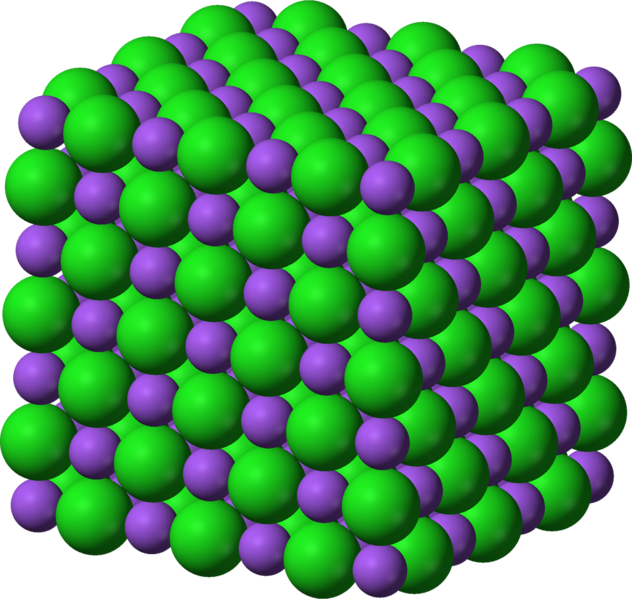
\includegraphics[width=0.5\textwidth]{photos/sodiumchloride_wikipedia.png}\\
\begin{caption}{'n Ruimtevullende model van die natrium chloriedrooster}\end{caption}
 \end{center}

\end{minipage}

      \label{m38684*uid71}
            \subsection*{Eienskappe van ioniese verbindings}
            \nopagebreak
Ioniese verbindings toon die volgende eienskappe:
        \label{m38684*id142815}\begin{itemize}[noitemsep]
            \label{m38684*uid72}\item Die ione word binne 'n kristalrooster gerangskik 
\label{m38684*uid73}\item Ioniese vaste stowwe is kristallyn (in kristalvorm) by kamertemperatuur
\label{m38684*uid74}\item Die ioniese binding is 'n sterk elektrostatiese aantrekkingskrag. Dit beteken dat ioniese verbindings meestal hard is en 'n ho\"{e} smelt- en kookpunt het
\label{m38684*uid75}\item Ioniese verbindings is bros en bindings breek gewoonlik by sekere plekke wanneer dit onder druk geplaas word
\label{m38684*uid76}\item Soliede kristalle gelei nie elektrisiteit nie, maar ioniese oplossings kan wel
\end{itemize}
\label{m38684*secfhsst!!!underscore!!!id522}
\begin{exercises}{Ioniese verbindings}
{
            \nopagebreak
        \label{m38684*id142562}\begin{enumerate}[noitemsep, label=\textbf{\arabic*}. ] 
            \label{m38684*uid57}\item Verduidelik die verskil tussen 'n kovalente en 'n ioniese binding.\newline
\label{m38684*uid58}\item Magnesium en chloor reageer om magnesiumchloried te vorm.
\label{m38684*id142602}\begin{enumerate}[noitemsep, label=\textbf{\alph*}. ] 
            \label{m38684*uid59}\item Wat is die verskil in elektronegatiwiteit tussen hierdie twee elemente?
\label{m38684*uid60}\item Gee die chemiese formule vir:
\label{m38684*id142630}\begin{enumerate}[noitemsep, label=\textbf{\roman*}. ] 
            \label{m38684*uid61}\item 'n magnesiumioon
\label{m38684*uid62}\item 'n chloriedioon
\label{m38684*uid63}\item die ioniese verbinding wat gevorm word tydens hierdie reaksie
\end{enumerate}
        \label{m38684*uid64}\item Skryf 'n gebalanseerde chemiese vergelyking neer vir die reaksie wat plaasvind.
\end{enumerate}
        \label{m38684*uid65}\item Teken Lewisdiagramme om die vorming van die volgende ioniese verbindings voor te stel:
\label{m38684*id142697}\begin{enumerate}[noitemsep, label=\textbf{\alph*}. ] 
            \label{m38684*uid66}\item natriumjodied  ($\text{NaI}$)
\label{m38684*uid67}\item kalsiumbromied ($\text{CaBr}{}_{2}$)
\label{m38684*uid68}\item kaliumchloried ($\text{KCl}$)

\end{enumerate}
        \end{enumerate}

\practiceinfo
\begin{tabular}[h]{cccccc}
 (1.) 025x  &  (2.) 025y  &  (3.) 025z  &
\end{tabular}
}
\end{exercises}

  \label{m38684**end}
         \section{Metaalbinding}
    \nopagebreak


            \subsection*{Die aard van metaalbinding}
            \nopagebreak
Die struktuur van 'n metaalbinding verskil baie van di\'e van kovalente en ioniese bindings. In 'n metaalbinding is die valenselektrone \textsl{gedelokaliseerd}, wat beteken dat die atoom se elektrone nie rondom die kern van die atoom bly nie. In 'n metaalbinding word die positiewe atoomkerne omring deur 'n see van gedelokaliseerde elektrone wat aangetrek word deur die kerne (Figuur 5,19).\\ 

\mindsetvid{A microscopic model of metals}{VPaxw}

\label{m38694*fhsst!!!underscore!!!id582}
\Definition{Metaalbinding} {Metaalbinding is die elektrostatiese aantrekkingskrag tussen die positief gelaaide atoomkerne van metaal-atome en die gedelokaliseerde elektrone in die metaal.}
\begin{minipage}{.5\textwidth}
    \setcounter{subfigure}{0}
% \begin{figure}[h]
\begin{center}
\scalebox{0.8}{
\begin{pspicture}(-3,-3)(3,3)
\psframe(0,0)(5,5)
%row 1
\multirput(1,1)(1,0){4}{
\pscircle(0,0){.2}
\uput[r]{0}(-0.3,0){$+$}}
%row 2
\pscircle(1,2){.2}
\uput[r]{0}(0.7,2){$+$}
\pscircle(2,2){.2}
\uput[r]{0}(1.7,2){$+$}
\pscircle(3,2){.2}
\uput[r]{0}(2.7,2){$+$}
\pscircle(4,2){.2}
\uput[r]{0}(3.7,2){$+$}
%row 3
\pscircle(1,3){.2}
\uput[r]{0}(0.7,3){$+$}
\pscircle(2,3){.2}
\uput[r]{0}(1.7,3){$+$}
\pscircle(3,3){.2}
\uput[r]{0}(2.7,3){$+$}
\pscircle(4,3){.2}
\uput[r]{0}(3.7,3){$+$}
%row 4
\pscircle(1,4){.2}
\uput[r]{0}(0.7,4){$+$}
\pscircle(2,4){.2}
\uput[r]{0}(1.7,4){$+$}
\pscircle(3,4){.2}
\uput[r]{0}(2.7,4){$+$}
\pscircle(4,4){.2}
\uput[r]{0}(3.7,4){$+$}
%the elektrons
\qdisk(0.2,0.5){1.5pt}
\qdisk(4.7,4.6){1.5pt}
\qdisk(1,4.5){1.5pt}
\qdisk(1.4,3.3){1.5pt}
\qdisk(2.8,1.7){1.5pt}
\qdisk(3.4,3){1.5pt}
\qdisk(4.3,3.2){1.5pt}
\qdisk(4.8,0.3){1.5pt}
\qdisk(2.5,2.5){1.5pt}
\qdisk(0.4,0.3){1.5pt}
\qdisk(1,0.6){1.5pt}
\qdisk(1.4,4.7){1.5pt}
\qdisk(0.6,2.1){1.5pt}
\qdisk(2.1,0.4){1.5pt}
\qdisk(3.4,0.7){1.5pt}
\qdisk(3,0.2){1.5pt}
\qdisk(4.5,0.4){1.5pt}
\qdisk(1.5,1.5){1.5pt}
\qdisk(0.3,3.7){1.5pt}
\qdisk(2.5,3.5){1.5pt}
\qdisk(4.7,1.5){1.5pt}
\qdisk(2.5,4.3){1.5pt}
\qdisk(3.2,4.4){1.5pt}
\qdisk(3.9,4.5){1.5pt}
\end{pspicture}
}
\end{center}
\begin{caption}{Positiewe atoomkerne (+) word omring deur gedelokaliseerde elektrone ($\bullet$)}\end{caption}
\label{fig:an:metallic bond}
% \end{figure}      
\end{minipage}
\begin{minipage}{.5\textwidth}
 \begin{center}
  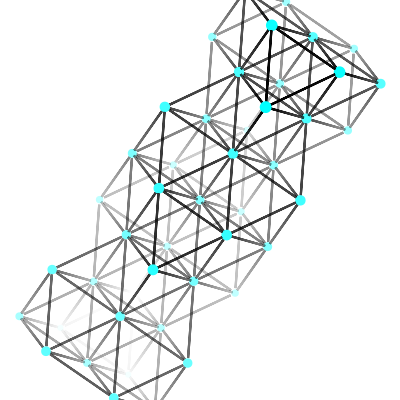
\includegraphics[width=0.6\textwidth]{photos/copper_structure.png}\\
\begin{caption}{Bal-en-stokmodel van koper}\end{caption}
 \end{center}

\end{minipage}
\subsection*{Eienskappe van metale}
\begin{enumerate}[noitemsep, label=\textbf{\arabic*}. ] 
 \item Metale het  'n \textsl{glans}.
\item Metale \textsl{gelei elektrisiteit} omdat die elektrone vry is om te beweeg.
\item Metale \textsl{gelei hitte} omdat die positiewe kerne teen mekaar saamgepak is en maklik hitte kan oordra.
\item Metale het 'n \textsl{ho\"{e} smeltpunt} omdat die bindings sterk is en 'n \textsl{ho\"{e} digtheid} as gevolg van die digte verpakking van die kerne (hulle is styf teenmekaar gepak).
\end{enumerate}

        \label{m38694*id754}
            \begin{activity}{Die bou van modelle}
     \begin{minipage}{.5\textwidth}
Deur gebruik te maak van gekleurde balle (of jellytots) en stokke (of tandestokkies) kan modelle gebou word van elke soort binding. Dink mooi hoe elke soort binding voorgestel kan word.  Kovalente binding kan byvoorbeeld voorgestel word deur bloot die koppeling van balle met stokkies om die molekules te verteenwoordig, terwyl vir ioniese binding jy  'n gedeelte van  'n kristalrooster kan bou. Doen  'n  bietjie navorsing oor verskillende tipes kristalroosters (hoewel die afdeling oor ioniese binding slegs die kristalrooster vir natriumchloried aantoon, bestaan daar baie ander vorme van roosters) en probeer om sommige van hulle te bou. Deel jou bevindinge met die res van die klas en vergelyk julle inligting om te sien watter tipes kristalroosters deur elkeen gevind is. Hoe sal jy metaalbinding voorstel?\par 
\end{minipage}
\begin{minipage}{.5\textwidth}
\scalebox{.6} % Change this value to rescale the drawing.
{
\begin{pspicture}(0,-4.44)(9.26,4.44)
\definecolor{color381b}{rgb}{0.8823529411764706,0.8823529411764706,0.8823529411764706}
\definecolor{color457b}{rgb}{0.7254901960784313,0.7254901960784313,0.7254901960784313}
\definecolor{color877}{rgb}{0.3137254901960784,0.3137254901960784,0.3137254901960784}
\definecolor{color878}{rgb}{0.47058823529411764,0.47058823529411764,0.47058823529411764}
\pspolygon[linewidth=0.04,fillstyle=solid,fillcolor=color381b](3.13,3.29)(4.11,4.25)(4.11,1.31)(3.13,0.33)
\pspolygon[linewidth=0.04,fillstyle=solid,fillcolor=color381b](0.17,3.31)(1.15,4.27)(1.15,1.33)(0.17,0.35)
\psframe[linewidth=0.04,dimen=outer,fillstyle=solid,fillcolor=color457b](4.13,4.31)(1.13,1.31)
\psframe[linewidth=0.04,dimen=outer](3.15,3.33)(0.15,0.33)
\psline[linewidth=0.04cm](3.13,3.31)(4.07,4.27)
\psdots[dotsize=0.3](1.15,1.35)
\psdots[dotsize=0.3](0.17,3.27)
\psdots[dotsize=0.3](1.13,4.25)
\psdots[dotsize=0.3](3.09,3.29)
\psdots[dotsize=0.3](4.07,4.27)
\psdots[dotsize=0.3](4.05,1.33)
\psdots[dotsize=0.3](0.17,0.37)
\psdots[dotsize=0.3](3.13,0.35)
\pspolygon[linewidth=0.04,fillstyle=solid,fillcolor=color381b](8.15,3.27)(9.13,4.23)(9.13,1.29)(8.15,0.31)
\pspolygon[linewidth=0.04,fillstyle=solid,fillcolor=color381b](5.19,3.29)(6.17,4.25)(6.17,1.31)(5.19,0.33)
\psframe[linewidth=0.04,dimen=outer,fillstyle=solid,fillcolor=color457b](9.15,4.29)(6.15,1.29)
\psframe[linewidth=0.04,dimen=outer](8.17,3.31)(5.17,0.31)
\psline[linewidth=0.04cm](8.15,3.29)(9.09,4.25)
\psdots[dotsize=0.3](6.17,1.33)
\psdots[dotsize=0.3](5.19,3.25)
\psdots[dotsize=0.3](6.15,4.23)
\psdots[dotsize=0.3](8.11,3.27)
\psdots[dotsize=0.3](9.09,4.25)
\psdots[dotsize=0.3](9.07,1.31)
\psdots[dotsize=0.3](5.21,0.33)
\pspolygon[linewidth=0.04,fillstyle=solid,fillcolor=color381b](5.13,-1.33)(6.11,-0.37)(6.11,-3.31)(5.13,-4.29)
\pspolygon[linewidth=0.04,fillstyle=solid,fillcolor=color381b](2.17,-1.31)(3.15,-0.35)(3.15,-3.29)(2.17,-4.27)
\psframe[linewidth=0.04,dimen=outer,fillstyle=solid,fillcolor=color457b](6.13,-0.31)(3.13,-3.31)
\psframe[linewidth=0.04,dimen=outer](5.15,-1.29)(2.15,-4.29)
\psline[linewidth=0.04cm](5.13,-1.31)(6.07,-0.35)
\psdots[dotsize=0.3](3.15,-3.27)
\psdots[dotsize=0.3](2.17,-1.35)
\psdots[dotsize=0.3](3.13,-0.37)
\psdots[dotsize=0.3](5.09,-1.33)
\psdots[dotsize=0.3](6.07,-0.35)
\psdots[dotsize=0.3](6.05,-3.29)
\psdots[dotsize=0.3](2.17,-4.25)
\psdots[dotsize=0.3](5.13,-4.27)
\psdots[dotsize=0.3](7.13,2.39)
\psdots[dotsize=0.3](8.17,0.33)
\psdots[dotsize=0.3,linecolor=color877](4.39,-1.97)
\psdots[dotsize=0.3,linecolor=color878](2.63,-2.27)
\psdots[dotsize=0.3,linecolor=color878](5.61,-2.17)
\psdots[dotsize=0.3](4.13,-0.81)
\psdots[dotsize=0.3](3.97,-3.81)
\psdots[dotsize=0.3](3.85,-2.47)
\end{pspicture} 
}
\end{minipage}
\end{activity}
% \label{m38694*eip-515}
%     \setcounter{subfigure}{0}
% 	\begin{figure}[H] % horizontal\label{m38694*bonds-1}
%     \textnormal{Khan academy video on bonding - 1}\vspace{.1in} \nopagebreak
%   \label{m38694*yt-media1}\label{m38694*yt-video1}
%             \raisebox{-5 pt}{ 
\includegraphics[width=0.5cm]{col11305.imgs/summary_www.png}} { (Video:  P10034 )}
%       \vspace{2pt}
%     \vspace{.1in}
%  \end{figure}       \par \label{m38694*secfhsst!!!underscore!!!id617}

\begin{exercises}{Verbindings}
{
            \nopagebreak
        \label{m38694*id143111}\begin{enumerate}[noitemsep, label=\textbf{\arabic*}. ] 
            \label{m38694*uid86}\item Gee twee voorbeelde van alledaagse voorwerpe wat die volgende bevat:
\label{m38694*id143127}\begin{enumerate}[noitemsep, label=\textbf{\alph*}. ] 
            \label{m38694*uid87}\item kovalente bindings
\label{m38694*uid88}\item ioniese bindings
\label{m38694*uid89}\item metaalbindings
\end{enumerate}
                \label{m38694*uid90}\item Voltooi die tabel om die verskillende tipes bindings te vergelyk:
    % \textbf{m38694*id143180}\par
          \begin{table}[H]
    % \begin{table}[H]
    % \\ 'id2900564' '1'
        \begin{center}
      \label{m38694*id143180}
    \noindent
      \begin{tabular}{|l|l|l|l|}\hline
         &
        \textbf{Kovalent} &
        \textbf{Ionies} &
        \textbf{Metaal} \\ \hline
        Tipes atome betrokke &
         &
         &
        \\ \hline
        Aard van die binding tussen atome &
         &
         &
       \\ \hline
        Smeltpunt (ho\"{e} / lae) &
         &
         &
       \\ \hline
        Elektrisiteit gelei? (Ja / Nee) &
         &
         &
      \\ \hline
        Ander eienskappe &
         &
         &
       \\ \hline
    \end{tabular}
      \end{center}
\end{table}
    \par
          \label{m38694*uid91}\item Voltooi die onderstaande tabel deur die identifisering van die tipe binding (kovalent-,  ionies- of  metaal) in elk van die verbindings:
    % \textbf{m38694*id143418}\par
          \begin{table}[H]
    % \begin{table}[H]
    % \\ 'id2900649' '1'
        \begin{center}
      \label{m38694*id143418}
    \noindent
      \begin{tabular}{|l|l|}\hline
        \textbf{Molekul\^{e}re formule } &
        \textbf{Tipe binding} \\ \hline
        $\text{H}_{2}\text{SO}_{4}$ &
        \\ \hline
        $\text{FeS}$ &
        \\ \hline
        $\text{NaI}$ &
         \\ \hline
        $\text{MgCl}_{2}$ &
        \\ \hline
        $\text{Zn}$ &
       \\ \hline
    \end{tabular}
      \end{center}
\end{table}
    \par

\label{m38694*uid93}\item Gebruik jou kennis van die verskillende tipes bindings om die volgende stellings te verduidelik.
\label{m38694*id143618}\begin{enumerate}[noitemsep, label=\textbf{\alph*}. ] 
            \label{m38694*uid94}\item 'n Natriumchloried kristal gelei nie elektrisiteit nie.
\label{m38694*uid95}\item Die meeste juweliersware word gemaak van metale.
\label{m38694*uid96}\item Dit is baie moeilik om 'n diamant te breek.
\item Potte word gemaak van metale, maar hulle handvatsels word van plastiek gemaak.
\end{enumerate}
                \end{enumerate}

\practiceinfo
\begin{tabular}[h]{cccccc}
 (1.) 0260  &  (2.) 0261  &  (3.) 0262  &  (4.) 0263  &  (5.) 0264  &
\end{tabular}
}
\end{exercises}


         \section{Die skryf van formules}
    \nopagebreak


In hoofstuk~\ref{chap:classification} het jy al iets geleer oor die skryf van chemiese formules. Tabel~\ref{tab:ions} toon 'n paar van die algemene anione en katione wat jy behoort te ken.
    % \textbf{m38689*uid99}\par
          \begin{table}[H]
    % \begin{table}[H]
    % \\ '' '0'
        \begin{center}
      \label{m38689*uid99}
    \noindent
      \begin{tabular}{|l|l|l|l|}\hline
                  \textbf{Naam van saamgestelde ioon} &
                  \textbf{formule} &  \textbf{Naam van saamgestelde ioon} & \textbf{formule} \\ \hline
        Karbonaat & $\mathrm{CO}_{3}^{2-}$ & Nitriet & $\mathrm{NO}_{2}^{-}$ \\ \hline
        Sulfaat &  $\mathrm{SO}_{4}^{2-}$ & Waterstof sulfiet & $\mathrm{HSO}_{3}^{-}$ \\ \hline
        Hidroksied & ${\mathrm{OH}}^{-}$ & Waterstof sulfaat & $\mathrm{HSO}_{4}^{-}$ \\ \hline
        Ammonium & $\mathrm{NH}_{4}^{+}$ & Dihidrogeenfosfaat & ${\mathrm{H}}_{2}\mathrm{PO}_{4}^{-}$ \\ \hline
        Nitraat & $\mathrm{NO}_{3}^{-}$ & Hipochloriet & ${\mathrm{ClO}}^{-}$ \\ \hline
        Waterstofkarbonaat & $\mathrm{HCO}_{3}^{-}$ & Asetaat (etanoaat)  & ${\mathrm{CH}}_{3}{\mathrm{COO}}^{-}$ \\ \hline
        Fosfaat & $\mathrm{PO}_{4}^{3-}$ & Oksalaat & ${\mathrm{C}}_{2}\mathrm{O}_{4}^{2-}$ \\ \hline
        Chloraat & $\mathrm{ClO}_{3}^{-}$ &  Oksied & ${\mathrm{O}}^{2-}$ \\ \hline
        Sianied & ${\mathrm{CN}}^{-}$ & Peroksied & $\mathrm{O}_{2}^{2-}$ \\ \hline
        Chromaat & $\mathrm{CrO}_{4}^{2-}$ & Sulfied & ${\mathrm{S}}^{2-}$ \\ \hline
        Permanganaat & $\mathrm{MnO}_{4}^{-}$ & Sulfiet & $\mathrm{SO}_{3}^{2-}$ \\ \hline
        Tiosulfaat & ${\mathrm{S}}_{2}\mathrm{O}_{3}^{2-}$ & Manganaat & $\mathrm{MnO}_{4}^{2-}$ \\ \hline
        Fosfied & ${\mathrm{P}}^{3-}$ & Waterstoffosfaat & $\mathrm{HPO}_{4}^{3-}$ \\ \hline
    \end{tabular}
      \end{center}
    \caption{Tabel met algemene saamgestelde ione en hul formules}
\label{tab:ions}
\end{table}
    \par
	\par

            \subsection*{Chemiese verbindings: name en massas}
            \nopagebreak
\label{m38689*uid97124}In hoofstuk~\ref{chap:atom} het jy iets geleer oor atoommassa. In hierdie hoofstuk het ons geleer dat atome kan verbind om verbindings te vorm. Molekules word gevorm wanneer atome kombineer deur middel van kovalente binding, 'n Ammoniakmolekuul, byvoorbeeld, bestaan ​​uit drie waterstofatome en een stikstofatoom. Die relatiewe molekul\^{e}re massa ($\textsf{M}$) van ammoniak ($\textsf{NH}_{3}$) is:\\
\begin{eqnarray*}
 \mbox{M} &=& \mbox{relatiewe atoommassa van een stikstofatoom} + \mbox{relatiewe atoommassa van drie waterstofatome}\\
&= & 14,0 + 3(1,01) \\
&= & 17,03
\end{eqnarray*}
Een molekuul $\textsf{NH}_{3}$ het dus  'n massa van van $17,03~\textsf{eenhede}$. Wanneer natrium reageer met chloor om natriumchloried te vorm, word daar nie een molekuul natriumchloried gevorm nie, maar eerder 'n natriumchloried kristalrooster. Onthou dat in ioniese binding molekules nie gevorm word nie. Ons kan ook die massa bereken van een eenheid van so 'n kristal. Ons noem dit 'n \textbf{formule-eenheid} en die massa is bekend as die \textbf{formulemassa}. Die formule-massa vir natriumchloried is
 \begin{eqnarray*}
 \mbox{M} &= &\mbox{relatiewe atoommassa van 'n natriumatoom} + \mbox{relatiewe atoommassa van 'n chlooratoom}\\
&= & 23,0 + 35,45 \\
&=& 58,45
\end{eqnarray*} 
Die formulemassa vir $\textsf{NaCl}$ is $58,45~\textsf{eenhede}$.
 

\begin{exercises}{Chemiese formulae }
{
            \nopagebreak
        \label{m38689*id145052}\begin{enumerate}[noitemsep, label=\textbf{\arabic*}. ] 
            \label{m38689*uid100}\item 
Voltooi die volgende tabel. Die katione aan die bokant verbind met die anione aan die linkerkant. Die eerste ry is reeds voltooi. Sluit ook die name van die verbindings wat gevorm word asook die anione in.
          \begin{table}[H]
        \begin{center}
      \label{m38689*id145067}
    \noindent
      \begin{tabular}{|p{1cm}|p{2.5cm}|p{2.5cm}|p{2.5cm}|p{2.5cm}|p{2.5cm}|}\hline
        &\textbf{ $\text{Na}^{+}$} & \textbf{$\text{Mg}^{2+}$} & \textbf{$\text{Al}^{3+}$} & \textbf{$\text{NH}_{4}^{+}$} & \textbf{$\text{H}^{+}$} \\ \hline
\multirow{2}{1cm}{\textbf{$\text{Br}^{-}$ naam:}} & $\text{NaBr}$  & $\text{MgBr}_2$  & $\text{AlBr}_3$  & $(\text{NH}_{4})\text{Br}$  & $\mathrm{HBr}$  \\ 
 & natriumbromied & magnesiumbromied & aluminiumbromied & ammoniumbromied & waterstofbromied \\ \hline
\textbf{$\text{S}^{2-}$ naam:} & & & & & \\ \hline
\textbf{$\text{P}^{3-}$ naam:} & & & & & \\ \hline
\textbf{$\text{MnO}_{4}^{-}$ naam:} & & & & & \\ \hline
\textbf{$\text{Cr}_{2}\text{O}_{7}^{2-}$ naam:} & & & & & \\ \hline
\textbf{$\text{HPO}_{4}^{2-}$ naam:} & & & & & \\ \hline
    \end{tabular}
      \end{center}
\end{table}
    \par
          \label{m38689*uid101}\item Skryf die chemiese formules neer vir elk van die volgende verbindings:
\label{m38689*id145444}\begin{enumerate}[noitemsep, label=\textbf{\alph*}. ] 
            \label{m38689*uid102}\item waterstofsianied
\label{m38689*uid103}\item koolstofdioksied
\label{m38689*uid104}\item natriumkarbonaat
\label{m38689*uid105}\item ammoniumhidroksied
\label{m38689*uid106}\item bariumsulfaat
\item koper(II)nitraat
\end{enumerate}
Bereken die relatiewe molekul\^{e}re massa of formulemassa vir elk van die verbindings hierbo.
                \end{enumerate}

\practiceinfo
\begin{tabular}[h]{cccccc}
 (1.) 0265  &  (2.) 0266  &
\end{tabular}
}
\end{exercises}
%     \label{m38689*eip-891}
%     \setcounter{subfigure}{0}
% 	\begin{figure}[H] % horizontal\label{m38689*slidesharefigure}
%     \label{m38689*slidesharemedia}\label{m38689*slideshareflash}\raisebox{-5 pt}{ 
\includegraphics[width=0.5cm]{col11305.imgs/summary_www.png}} { (Presentation:  P10036 )}
%       \vspace{2pt}
%     \vspace{.1in}
%  \end{figure}       \par \label{m38689*cid13}

\summary{VPduz}
            \nopagebreak
\begin{itemize}[noitemsep]
\item 'n \textbf{Chemiese binding} is 'n fisiese proses wat veroorsaak dat atome en molekule mekaar aantrek en bymekaar gehou word in meer stabiele verbindings.
\item Atome is meer \textbf{reaktief}, en dus meer geneig om bindings te vorm wanneer hulle buitenste elektron orbitale nie gevul is nie. Atome is minder reaktief wanneer hierdie buitenste orbitale die maksimum aantal elektrone bevat. Dit verklaar waarom die edelgasse nie reaktief is nie.
\item Wanneer atome bind, word elektrone gedeel of uitgeruil.
\item \textbf{Kovalente binding} vind plaas tussen die atome van nie-metale en behels die deel van elektrone sodat orbitale van die buitenste energievlakke in die atome gevul is.
\item 'n \textbf{Dubbel}- of \textbf{trippelbinding} vind plaas wanneer daar twee of drie elektronpare gedeel word tussen die twee atome.
\item \textbf{Lewis}notasie is een manier waarop molekulêrestruktuur voorgestel kan word. In Lewisnotasie word kolletjies en kruisies gebruik om die valenselektrone rondom die sentrale atoom te verteenwoordig.
\item 'n \textbf{Ioniese binding} tussen atome kom voor waar daar 'n groot verskil in elektronegatiwiteit bestaan. 'n Uitruiling van elektrone vind plaas en die atome word bymekaar gehou deur die elektrostatiese  aantrekkingskrag tussen teenoorgesteld gelaaide ione.
\item Ioniese vaste stowwe is gerangskik binne 'n \textbf{kristalrooster}struktuur.
\item Ioniese verbindings het 'n aantal spesifieke \textbf{eienskappe}, insluitend hul hoë smelt-en kookpunte, bros natuur, die kristalroosterstruktuur van vaste stowwe en die vermo\"{e} van ioniese oplossings om elektrisiteit te gelei.
\item 'n \textbf{Metaalbinding} is die elektrostatiese aantrekkingskrag tussen die positief gelaaide kerne van metaalatome en die gedelokaliseerde elektrone in die metaal.
\item Metale het ook 'n aantal eienskappe, insluitend hul vermo\"{e} om hitte en elektrisiteit te gelei, hul metaalglans, die feit dat hulle pletbaar en buigbaar is en dat hul ho\"{e} smeltpunte en digtheid besit.
\item Die valenselektrone van atome en die wyse waarop hulle bind kan gebruik word om die \textbf{chemiese formules} vir verbindings te bepaal.
\end{itemize}
\label{m38689*secfhsst!!!underscore!!!id1181}
            \begin{eocexercises}{Chemiese binding}
            \nopagebreak
      \label{m38689*id147820}\begin{enumerate}[noitemsep, label=\textbf{\arabic*}. ] 
            \label{m38689*uid158}\item Verduidelik die betekenis van elk van die volgende terme
\label{m38689*id147842}\begin{enumerate}[noitemsep, label=\textbf{\alph*}. ] 
            \label{m38689*uid159}\item Ioniese binding
\label{m38689*uid160}\item Kovalente binding
\end{enumerate}
                \label{m38689*uid162}\item Watter EEN van die volgende is die beste beskrywing vir die binding tussen koolstof en waterstof?
\label{m38689*id147923}\begin{enumerate}[noitemsep, label=\textbf{\alph*}. ] 
            \label{m38689*uid163}\item metaalbinding
\label{m38689*uid164}\item kovalente binding
\label{m38689*uid165}\item ioniese binding
\end{enumerate}
                \label{m38689*uid171}\item Watter een van die volgende reaksies sal nie plaasvind nie? Verduidelik jou antwoord.
\label{m38689*id148047}\begin{enumerate}[noitemsep, label=\textbf{\alph*}. ] 
            \label{m38689*uid172}\item $\mathrm{H}+\mathrm{H}\to {\mathrm{H}}_{2}$\label{m38689*uid173}\item $\mathrm{Ne}+\mathrm{Ne}\to {\mathrm{Ne}}_{2}$\label{m38689*uid174}\item $\mathrm{Cl}+\mathrm{Cl}\to {\mathrm{Cl}}_{2}$\end{enumerate}
                \label{m38689*uid175}\item Teken die Lewisstruktuur vir die vorming van elk van die volgende:
\label{m38689*id148172}\begin{enumerate}[noitemsep, label=\textbf{\alph*}. ] 
            \label{m38689*uid176}\item kalsiumchloried
\label{m38689*uid177}\item jodiumgas ($\text{I}_2$)
\label{m38689*uid178}\item waterstofbromied ($\text{HBr}$)
\label{m38689*uid179}\item stikstofdioksied ($\text{NO}{}_{2}$)
\end{enumerate}
                \label{m38689*uid180}\item Gegewe die volgende Lewisstruktuur, waar X en Y elk  'n ander element verteenwoordig ...
    \setcounter{subfigure}{0}
	\begin{figure}[H] % horizontal\label{m38689*id148255}
\begin{center}
\begin{pspicture}(-2,-0.8)(3,0.6)
%\psgrid[gridcolor=gray]
\rput(-0.3,0){\Large \textbf{X}}
\rput(0.6,0){\Large \textbf{Y}}
\rput(1.5,0){\Large \textbf{X}}
\rput(0.6,-0.9){\Large \textbf{X}}

\rput{90}(0.6,0){\uput{9pt}[d](0,0){$\times$ $\bullet$}}
\rput{270}(0.6,0){\uput{9pt}[d](0,0){$\times$ $\bullet$}}
\uput{9pt}[u](0.6,0){$\times$ $\times$}
\uput{9pt}[d](0.6,0){$\times$ $\bullet$}
\end{pspicture}
\end{center}
 \end{figure}      

 \label{m38689*id148261}\begin{enumerate}[noitemsep, label=\textbf{\alph*}. ] 
            \label{m38689*uid181}\item Wat is die valensie van $\mathrm{X}$?
\label{m38689*uid182}\item Wat is die valensie van  $\mathrm{Y}$?
\label{m38689*uid183}\item Watter elemente kan moontlik $\mathrm{X}$ en $\mathrm{Y}$ verteenwoordig?
\end{enumerate}
\item Voltooi die volgende tabel:
\begin{table}[H]
\begin{center}
 \begin{tabular}{|l|l|l|l|} \hline
  & \textbf{$\text{K}^{+}$} & \textbf{$\text{Ca}^{2+}$} & \textbf{$\text{NH}_{4}^{+}$} \\ \hline
\textbf{$\text{OH}^{-}$} & & & \\ \hline   
\textbf{$\text{O}^{2-}$} & & & \\ \hline   
\textbf{$\text{NO}_{3}^{-}$} & & & \\ \hline   
\textbf{$\text{PO}_{4}^{3-}$} & & & \\ \hline   
 \end{tabular}
\end{center}
\end{table}

              \label{m38689*uid185}\item Kaliumdichromaat los op in water.
\label{m38689*id148361}\begin{enumerate}[noitemsep, label=\textbf{\alph*}. ] 
            \label{m38689*uid186}\item Gee die naam en die chemiese formule vir elk van die ione in die oplossing.
\label{m38689*uid187}\item Wat is die chemiese formule vir kaliumdichromaat?
\end{enumerate}
                \end{enumerate}

\practiceinfo
\begin{tabular}[h]{cccccc}
 (1.) 0267  &  (2.) 0268  &  (3.) 0269  &  (4.) 026a  &  (5.) 026b  &  (6.) 026c  &  (7.) 026d  &
\end{tabular}
\end{eocexercises}
